\section{Experiments}
We evaluate the representation learning capabilities of ResNet, \oursfull{} (\oursabbrv{}), and the hybrid.
To understand the data requirements of each model, we pre-train on datasets of varying size and evaluate many benchmark tasks.
When considering the computational cost of pre-training the model, \oursabbrv{} performs very favourably, attaining state of the art on most recognition benchmarks at a lower pre-training cost.
Lastly, we perform a small experiment using self-supervision, and show that self-supervised \oursabbrv{} holds promise for the future.

\subsection{Setup}

\textbf{Datasets.}
To explore model scalability, we use the ILSVRC-2012 ImageNet dataset with 1k classes and 1.3M images (we refer to it as \imagenet in what follows),
its superset ImageNet-21k with 21k classes and 14M images~\citep{deng2009-imagenet},
and JFT~\citep{sun2017-jft} with  18k classes and 303M high-resolution images.
We de-duplicate the pre-training datasets w.r.t. the test sets of the downstream tasks following~\citet{kolesnikov2020-bit}.
We transfer the models trained on these dataset to several benchmark tasks:
\imagenet on the original validation labels and the cleaned-up ReaL labels~\citep{beyer2020-imagenet},
CIFAR-10/100~\citep{Krizhevsky2009-cifar}, 
Oxford-IIIT Pets~\citep{parkhi2012-pets}, 
and  Oxford Flowers-102~\citep{Nilsback2008-flowers}.
For these datasets, pre-processing follows \citet{kolesnikov2020-bit}.

We also evaluate on the 19-task VTAB classification suite~\citep{vtab}.
VTAB evaluates low-data transfer to diverse tasks, using 1\,000 training examples per task.
The tasks are divided into three groups: 
\textit{Natural} -- tasks like the above, Pets, CIFAR, etc.
\textit{Specialized} -- medical and satellite imagery, and
\textit{Structured} -- tasks that require geometric understanding like localization.

\textbf{Model Variants.}
We base \oursabbrv{} configurations on those used for BERT~\citep{devlin19-bert}, as summarized in Table~\ref{tbl:models}. 
The ``Base'' and ``Large'' models are directly adopted from BERT and we add the larger ``Huge'' model.
In what follows we use brief notation to indicate the model size and the input patch size: for instance, \oursabbrv{}-L/16 means the ``Large'' variant with $16\times 16$ input patch size.
Note that the Transformer's sequence length is inversely proportional to the square of the patch size, thus models with smaller patch size are computationally more expensive.

For the baseline CNNs, we use ResNet~\citep{he2016deep}, but replace the Batch Normalization layers~\citep{ioffe2015batch} with Group Normalization~\citep{wu2018group}, and used standardized convolutions~\citep{qiao2019ws}.
These modifications improve transfer~\citep{kolesnikov2020-bit}, and we denote the modified model ``ResNet (BiT)''.
For the hybrids, we feed the intermediate feature maps into \oursabbrv{} with patch size of one ``pixel''.
To experiment with different sequence lengths, we either
(i) take the output of stage 4 of a regular ResNet50 or
(ii) remove stage 4, place the same number of layers in stage 3 (keeping the total number of layers), and take the output of this extended stage 3.
Option (ii) results in a 4x longer sequence length, and a more expensive \oursabbrv{} model.

\begin{table}[t]
\centering
\small
\begin{tabular}{l c c c c c}
\toprule
Model            & Layers & Hidden size $D$ & MLP size &  Heads  & Params \\
\midrule 
\oursabbrv-Base   &   12   &        768      &   3072   &   12    &   86M  \\
\oursabbrv-Large  &   24   &       1024      &   4096   &   16    &  307M  \\
\oursabbrv-Huge   &   32   &       1280      &   5120   &   16    &  632M  \\
\bottomrule
\end{tabular}
\caption{Details of \oursfull model variants.}
\label{tbl:models}
\end{table}

\textbf{Training \& Fine-tuning.}
We train all models, including ResNets, using Adam~\citep{kingma2015adam} with $\beta_1=0.9$, $\beta_2=0.999$, a batch size of 4096 and apply a high weight decay of $0.1$, which we found to be useful for transfer of all models (Appendix~\ref{sec:sgd_vs_adam} shows that, in contrast to common practices, Adam works slightly better than SGD for ResNets in our setting).
We use a linear learning rate warmup and decay, see Appendix~\ref{sec:training} for details.
For fine-tuning we use SGD with momentum, batch size 512, for all models, see Appendix~\ref{sec:finetuning}.
For \imagenet results in Table~\ref{tbl:best_results}, we fine-tuned at higher resolution: $512$ for \oursabbrv-L/16 and $518$ for \oursabbrv-H/14, and also used \citet{polyak} averaging with a factor of $0.9999$~\citep{ramachandran19-sasa,wang2020axial}.


\textbf{Metrics.}
We report results on downstream datasets either through few-shot or fine-tuning accuracy.
Fine-tuning accuracies capture the performance of each model after fine-tuning it on the respective dataset.
Few-shot accuracies are obtained by solving a regularized least-squares regression problem that maps the (frozen) representation of a subset of training images to $\{-1,1\}^K$ target vectors.
This formulation allows us to recover the exact solution in closed form.
Though we mainly focus on fine-tuning performance, we sometimes use linear few-shot accuracies for fast on-the-fly evaluation where fine-tuning would be too costly.

\subsection{Comparison to State of the Art}

We first compare our largest models~-- \oursabbrv-H/14 and \oursabbrv-L/16 ~-- to state-of-the-art CNNs from the literature.
The first comparison point is Big Transfer (BiT)~\citep{kolesnikov2020-bit}, which performs supervised transfer learning with large ResNets.
The second is Noisy Student~\citep{xie2020-noisystudent},
which is a large EfficientNet trained using semi-supervised learning on \imagenet and JFT-300M with the labels removed.
Currently, Noisy Student is the state of the art on \imagenet and BiT-L on the other datasets reported here.
All models were trained on TPUv3 hardware, and we report the number of TPUv3-core-days taken to pre-train each of them, that is, the number of TPU v3 cores (2 per chip) used for training multiplied by the training time in days.

\begin{table}[t]
\centering
\resizebox{\textwidth}{!}{
\begin{tabular}{l c c c c c}
\toprule
                   & Ours-JFT                & Ours-JFT              & Ours-I21k             & BiT-L                 & Noisy Student    \\
                   & (\oursabbrv-H/14)       & (\oursabbrv-L/16)     & (\oursabbrv-L/16)     & (ResNet152x4)         & (EfficientNet-L2)    \\
\midrule 
\imagenet          & \valstdb{88.55}{0.04}   & \valstd{87.76}{0.03}  & \valstd{85.30}{0.02}  & \valstd{87.54}{0.02}  &  $88.4/88.5^*$           \\
\imagenet ReaL     & \valstdb{90.72}{0.05}   & \valstd{90.54}{0.03}  & \valstd{88.62}{0.05}  & $90.54$               &  $90.55$          \\
CIFAR-10           & \valstdb{99.50}{0.06}   & \valstd{99.42}{0.03}  & \valstd{99.15}{0.03}  & \valstd{99.37}{0.06}  &  $-$              \\
CIFAR-100          & \valstdb{94.55}{0.04}   & \valstd{93.90}{0.05}  & \valstd{93.25}{0.05}  & \valstd{93.51}{0.08}  &  $-$              \\
Oxford-IIIT Pets   & \valstdb{97.56}{0.03}   & \valstd{97.32}{0.11}  & \valstd{94.67}{0.15}  & \valstd{96.62}{0.23}  &  $-$              \\
Oxford Flowers-102 & \valstd{99.68}{0.02}    & \valstdb{99.74}{0.00} & \valstd{99.61}{0.02}  & \valstd{99.63}{0.03}  &  $-$              \\
VTAB (19 tasks)    & \valstdb{77.63}{0.23}   & \valstd{76.28}{0.46}  & \valstd{72.72}{0.21}    & \valstd{76.29}{1.70}  &  $-$              \\
\midrule 
TPUv3-core-days    & $2.5$k                  & $0.68$k               & $0.23$k               & $9.9$k                &  $12.3$k           \\
\bottomrule
\end{tabular}
}
\caption{
Comparison with state of the art on popular image classification benchmarks.
We report mean and standard deviation of the accuracies, averaged over three fine-tuning runs.
\oursfull models pre-trained on the JFT-300M dataset outperform ResNet-based baselines on all datasets, while taking substantially less computational resources to pre-train.
\oursabbrv pre-trained on the smaller public ImageNet-21k dataset performs well too.
$^*$Slightly improved $88.5\%$ result reported in~\citet{touvron2020}.}
\label{tbl:best_results}
\end{table}

\begin{figure}[]
\begin{center}
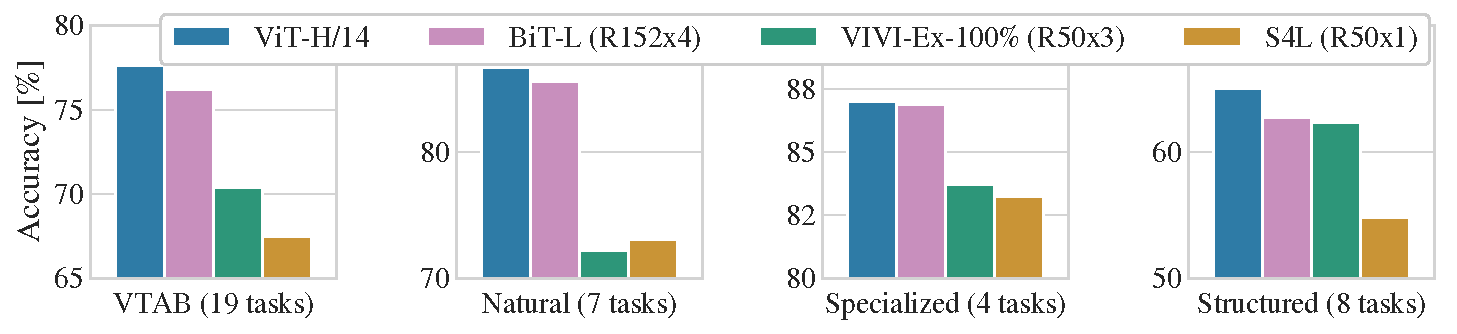
\includegraphics[width=0.98\textwidth]{images/vit-vtab.pdf}
\end{center}
\caption{Breakdown of VTAB performance in \textit{Natural}, \textit{Specialized}, and \textit{Structured} task groups. 
}
\label{fig:vtab}
\vspace{-3mm}
\end{figure}


Table~\ref{tbl:best_results} shows the results.
The smaller \oursabbrv-L/16 model pre-trained on JFT-300M outperforms BiT-L (which is pre-trained on the same dataset) on all tasks, while requiring substantially less computational resources to train.
The larger model, \oursabbrv-H/14, further improves the performance, especially on the more challenging datasets~-- \imagenet, CIFAR-100, and the VTAB suite.
Interestingly, this model still took substantially less compute to pre-train than prior state of the art. However, we note that pre-training efficiency may be affected not only by the architecture choice, but also other parameters, such as training schedule, optimizer, weight decay, etc.
We provide a controlled study of performance vs. compute for different architectures in Section~\ref{sec:scaling_architectures}.
Finally, the \oursabbrv-L/16 model pre-trained on the public ImageNet-21k dataset performs well on most datasets too, while taking fewer resources to pre-train: it could be trained using a standard cloud TPUv3 with 8 cores in approximately 30 days.

Figure~\ref{fig:vtab} decomposes the VTAB tasks into their respective groups, and compares to previous SOTA methods on this benchmark:
BiT,
VIVI -- a ResNet co-trained on \imagenet and Youtube~\citep{vivi},
and S4L -- supervised plus semi-supervised learning on \imagenet~\citep{zhai2019s4l}.
\oursabbrv{}-H/14 outperforms BiT-R152x4, and other methods, on the \textit{Natural} and \textit{Structured} tasks.
On the \textit{Specialized} the performance of the top two models is similar.

\subsection{Pre-training Data Requirements}
\label{sec:data_efficiency}

\begin{figure}
    \begin{minipage}[t]{0.47\textwidth}
        \centering
        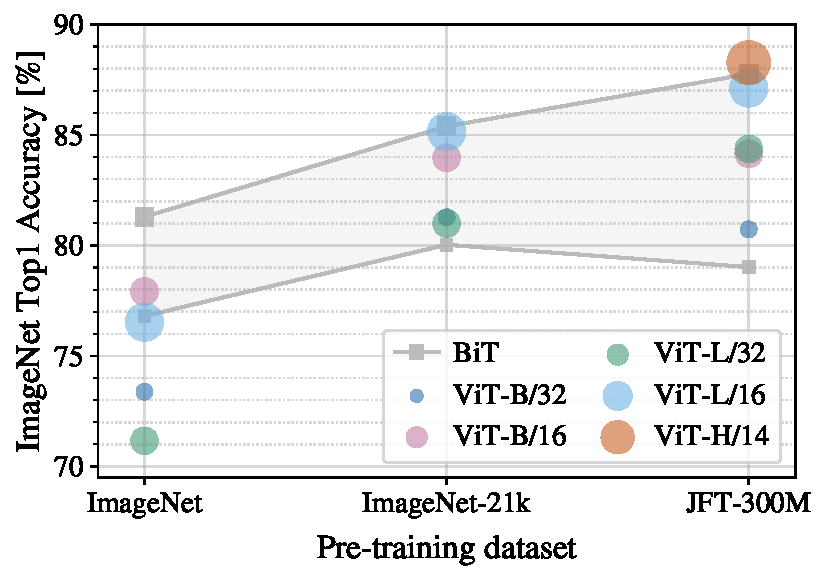
\includegraphics[width=1.0\textwidth]{images/dataset_analysis/transvolution-i1k-scaling}
        \caption{Transfer to \imagenet. While large \oursabbrv{} models perform worse than BiT ResNets (shaded area) when pre-trained on small datasets, they shine when pre-trained on larger datasets. Similarly, larger \oursabbrv{}  variants overtake smaller ones as the dataset grows.}
        \label{fig:imagenet_imagenet21k_jft}
    \end{minipage}\;\;\;\;
    \begin{minipage}[t]{0.47\textwidth}
        \centering
        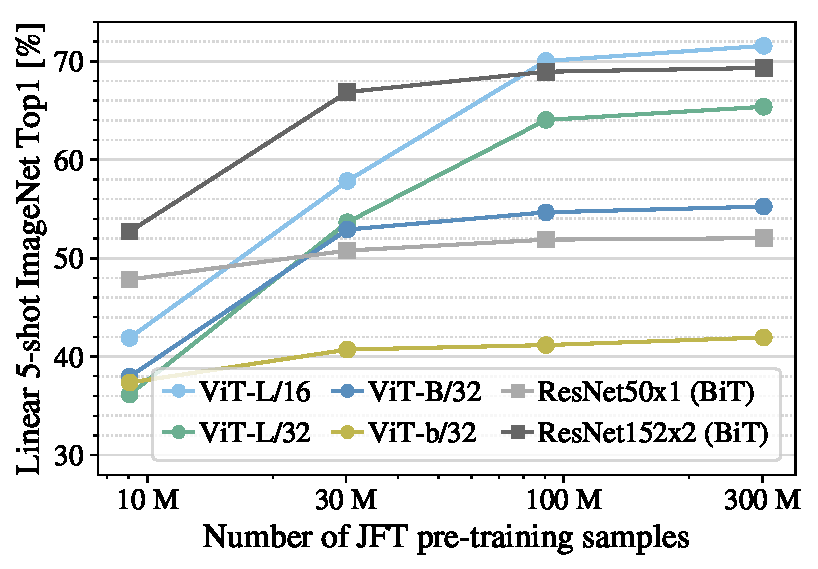
\includegraphics[width=1.0\textwidth]{images/dataset_analysis/imagenet_5shot}
        \caption{Linear few-shot evaluation on ImageNet versus pre-training size. 
        ResNets perform better with smaller pre-training datasets but plateau sooner than \oursabbrv{}, which performs better with larger pre-training. \oursabbrv-b is \oursabbrv-B with all hidden dimensions halved.}
        \label{fig:jft_amount_of_data}
    \end{minipage}
    \vspace{-3mm}
\end{figure}

The \oursfull performs well when pre-trained on a large JFT-300M dataset. 
With fewer inductive biases for vision than ResNets, how crucial is the dataset size?
We perform two series of experiments.

First, we pre-train \oursabbrv{} models on datasets of increasing size: \imagenet, ImageNet-21k, and JFT-300M.
To boost the performance on the smaller datasets, we optimize three basic regularization parameters~-- weight decay, dropout, and label smoothing.
Figure~\ref{fig:imagenet_imagenet21k_jft} shows the results after fine-tuning to \imagenet (results on other datasets are shown in Table~\ref{tbl:imagenet_imagenet21k_jft})\footnote{Note that the \imagenet pre-trained models are also fine-tuned, but again on \imagenet. This is because the resolution increase during fine-tuning improves the performance.}.
When pre-trained on  the smallest dataset, \imagenet, \oursabbrv{}-Large models underperform compared to \oursabbrv{}-Base models, despite (moderate) regularization.
With ImageNet-21k pre-training, their  performances are similar.
Only with JFT-300M, do we see the full benefit of larger models.
Figure~\ref{fig:imagenet_imagenet21k_jft} also shows the performance region spanned by BiT models of different sizes.
The BiT CNNs outperform \oursabbrv{} on \imagenet, but with the larger datasets, \oursabbrv{} overtakes.

Second, we train our models on random subsets of 9M, 30M, and 90M as well as the full JFT-300M dataset.
We do not perform additional regularization on the smaller subsets and use the same hyper-parameters for all settings.
This way, we assess the intrinsic model properties, and not the effect of regularization.
We do, however, use early-stopping, and report the best validation accuracy achieved during training.
To save compute, we report few-shot linear accuracy instead of full fine-tuning accuracy.
Figure~\ref{fig:jft_amount_of_data} contains the results.
\oursfull{}s overfit more than ResNets with comparable computational cost on smaller datasets. 
For example, \oursabbrv-B/32 is slightly faster than ResNet50; it performs much worse on the 9M subset, but better on 90M+ subsets.
The same is true for ResNet152x2 and \oursabbrv-L/16.
This result reinforces the intuition that the convolutional inductive bias is useful for smaller datasets, but for larger ones, learning the relevant patterns directly from data is sufficient, even beneficial.

Overall, the few-shot results on ImageNet (Figure~\ref{fig:jft_amount_of_data}), as well as the low-data results on VTAB (Table~\ref{tbl:best_results}) seem promising for very low-data transfer. Further analysis of few-shot properties of \oursabbrv{} is an exciting direction of future work.






\begin{figure}
\begin{center}
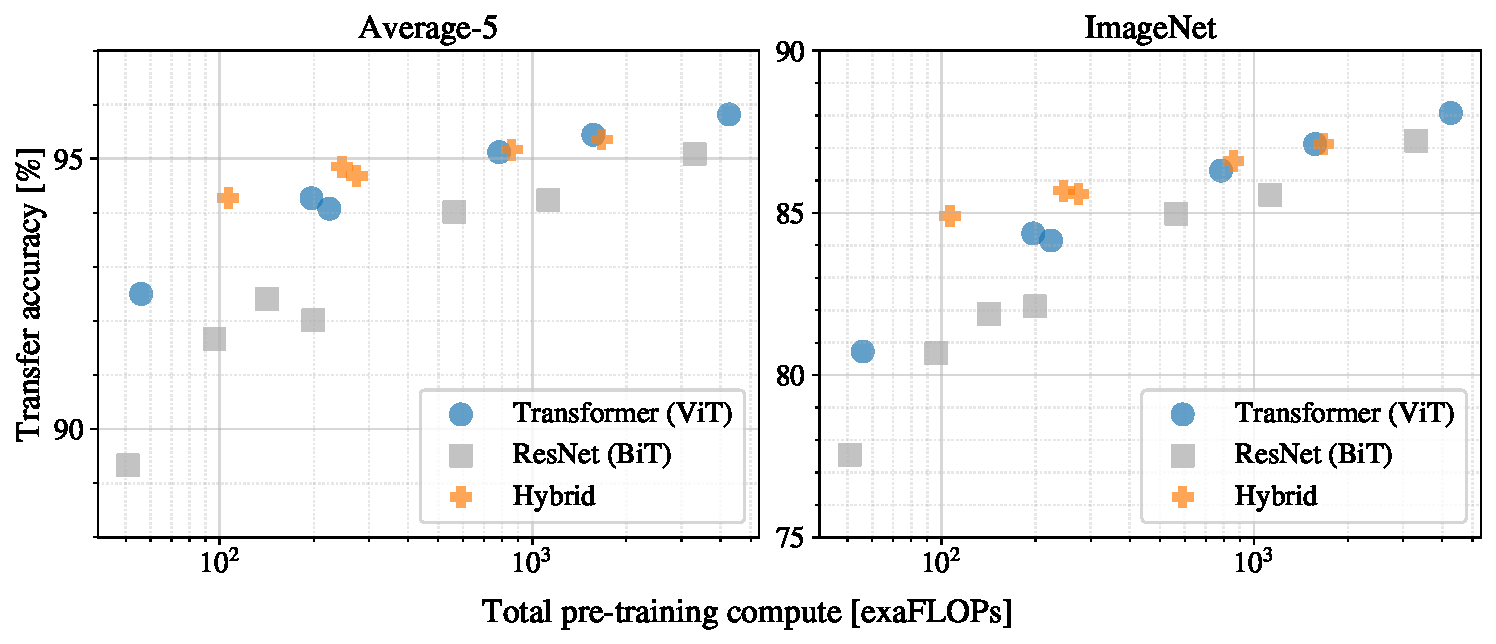
\includegraphics[width=0.92\textwidth]{images/finetune_vs_compute2}
\vspace{-3mm}
\end{center}
\caption{Performance versus pre-training compute for different architectures: \oursfull{}s, ResNets, and hybrids. \oursfull{}s generally outperform ResNets with the same computational budget. Hybrids improve upon pure Transformers for smaller model sizes, but the gap vanishes for larger models.}
\vspace{-3mm}
\label{fig:scaling_architectures}
\end{figure}

\subsection{Scaling Study}
\label{sec:scaling_architectures}

We perform a controlled scaling study of different models by evaluating transfer performance from JFT-300M.
In this setting data size does not bottleneck the models' performances, and we assess performance versus pre-training cost of each model.
The model set includes: 
7 ResNets, R50x1, R50x2 R101x1, R152x1, R152x2, pre-trained for 7 epochs, plus R152x2 and R200x3 pre-trained for 14 epochs;
6 \oursfull{}s, \oursabbrv-B/32, B/16, L/32, L/16, pre-trained for 7 epochs, plus L/16 and H/14 pre-trained for 14 epochs;
and 5 hybrids, R50+\oursabbrv-B/32, B/16, L/32, L/16 pre-trained for 7 epochs, plus R50+\oursabbrv-L/16 pre-trained for 14 epochs (for hybrids, the number at the end of the model name stands not for the patch size, but for the total dowsampling ratio in the ResNet backbone).

Figure~\ref{fig:scaling_architectures} contains the transfer performance versus  total pre-training compute (see  Appendix~\ref{sec:empirical_computation} for details on computational costs).
Detailed results per model are provided in Table~\ref{tbl:scaling_architectures} in the Appendix.
A few patterns can be observed.
First, \oursfull{}s dominate ResNets on the performance/compute trade-off.
\oursabbrv{} uses approximately $2-4\times$ less compute to attain the same performance (average over 5 datasets).
Second, hybrids slightly outperform \oursabbrv{} at small computational budgets, but the difference vanishes for larger models.
This result is somewhat surprising, since one might expect convolutional local feature processing to assist \oursabbrv{} at any size.
Third, \oursfull{}s appear not to saturate within the range tried, motivating future scaling efforts.



\subsection{Inspecting \oursfull{}}
\begin{wrapfigure}{r}{0.3\textwidth}
\centering
\vspace{-2.7mm}
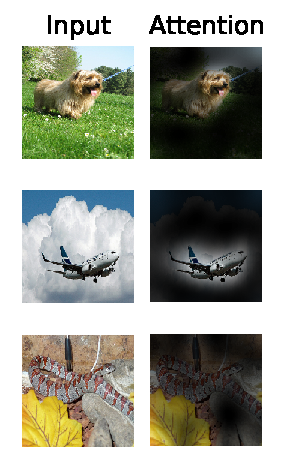
\includegraphics[height=2.5in,trim={0in 0in 0.15in 0in},clip]{images/visualizations/20201002_selected_attention_examples.pdf}
\caption{Representative examples of attention from the output token to the input space. See Appendix~\ref{sec:appendix_attention_distance} for details.}
\label{fig:selected_attention_examples}
\vspace{-4mm}
\end{wrapfigure}
To begin to understand how the \oursfull{} processes image data, we analyze its internal representations.
The first layer of the \oursfull{} linearly projects the flattened patches into a lower-dimensional space (Eq.~\ref{eq:embedding}). 
Figure~\ref{fig:transformer_visualization} (left) shows the top principal components of the the learned embedding filters. 
The components resemble plausible basis functions for a low-dimensional representation of the fine structure within each patch.

After the projection, a learned position embedding is added to the  patch representations. 
Figure~\ref{fig:transformer_visualization} (center) shows that the model learns to encode distance within the image in the similarity of position embeddings, i.e. closer patches tend to have more similar position embeddings. 
Further, the row-column structure appears; patches in the same row/column have similar embeddings.
Finally, a sinusoidal structure is sometimes apparent for larger grids (Appendix~\ref{sec:additional_analyses}). 
That the position embeddings learn to represent 2D image topology explains why hand-crafted 2D-aware embedding variants do not yield improvements (Appendix~\ref{app:pos_emb}).

\begin{figure}[t]
\vspace{3mm}
    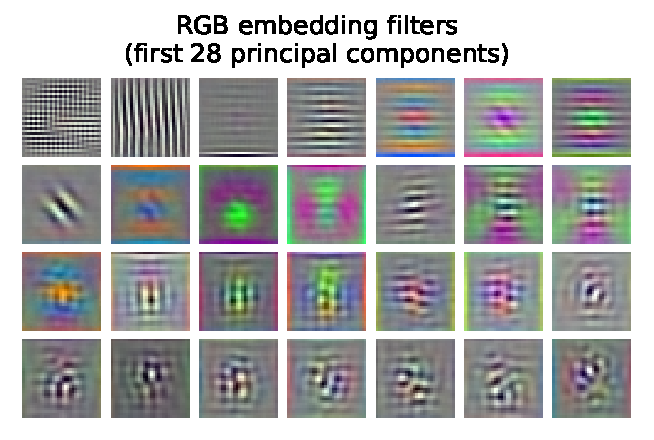
\includegraphics[height=1.5in,trim={0.15in 0in 0in 0in},clip]{images/visualizations/20201002_rgb_filter_pca.pdf}
    \hfill
    \raisebox{-0.15in}{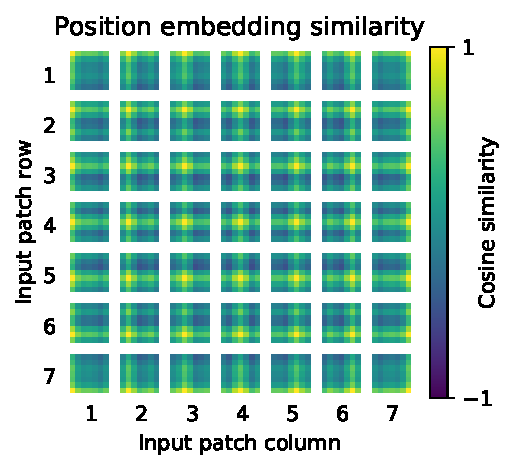
\includegraphics[height=1.5in]{images/visualizations/20201002_position_embeddings_17085772_1.pdf}}
    \hfill
    \raisebox{-0.15in}{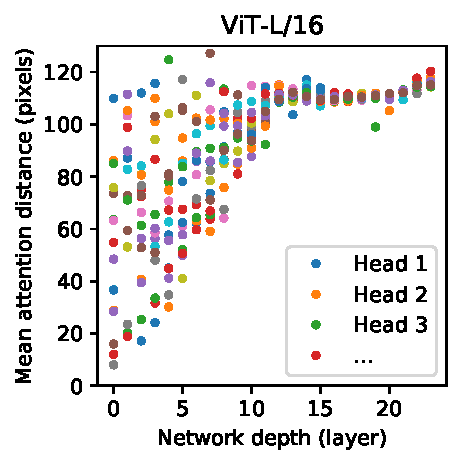
\includegraphics[height=1.5in,trim={0in 0in 0in 0in},clip]{images/visualizations/20201002_attention_distance_by_depth_main.pdf}}
    \caption{
        \textbf{Left:} Filters of the initial linear embedding of RGB values of \oursabbrv-L/32.
        \textbf{Center:} Similarity of position embeddings of \oursabbrv-L/32. Tiles show the cosine similarity between the position embedding of the patch with the indicated row and column and the position embeddings of all other patches.
        \textbf{Right:} Size of attended area by head and network depth. Each dot shows the mean attention distance across images for one of 16 heads at one layer. See Appendix~\ref{sec:appendix_attention_distance} for details.}
    \label{fig:transformer_visualization}
    \vspace{5mm}
\end{figure}

Self-attention allows \oursabbrv to integrate information across the entire image even in the lowest layers. We investigate to what degree the network makes use of this capability. Specifically, we compute the average distance in image space across which information is integrated, based on the attention weights (Figure~\ref{fig:transformer_visualization}, right). This ``attention distance'' is analogous to receptive field size in CNNs. We find that some heads attend to most of the image already in the lowest layers, showing that the ability to integrate information globally is indeed used by the model. Other attention heads have consistently small attention distances in the low layers. This highly localized attention is less pronounced in hybrid models that apply a ResNet before the Transformer (Figure~\ref{fig:transformer_visualization}, right), suggesting that it may serve a similar function as early convolutional layers in CNNs. 
Further, the attention distance increases with network depth.
Globally, we find that the model attends to image regions that are semantically relevant for classification (Figure~\ref{fig:selected_attention_examples}).


\subsection{Self-supervision}
Transformers show impressive performance on NLP tasks. However, much of their success stems not only from their excellent scalability but also from large scale self-supervised pre-training \citep{devlin19-bert,radford2018-gpt}. We also perform a preliminary exploration on \textit{masked patch prediction} for self-supervision, mimicking the masked language modeling task used in BERT. With self-supervised pre-training, our smaller \oursabbrv-B/16 model achieves 79.9\% accuracy on \imagenet{}, a significant improvement of 2\% to training from scratch, but still 4\% behind supervised pre-training. Appendix~\ref{sec:self_supervision} contains further details.
We leave exploration of contrastive pre-training \citep{Chen2020simclr,he2020moco,bachman2019amdim,henaff2020cpc} to future work.




